%%% LearnPAd Document template / example using learnpad.cls class for styling
%%% 20140401, 
%%% Guglielmo De Angelis <guglielmo.deangelis@isti.cnr.it>
%%% Andrea Polini <andrea.polini@unicam.it>

\documentclass{learnpad}
\usepackage[showtodos,showcomments]{labsedc}
\usepackage{extracommands}

%%% ------------------------------------------------------
%%% ---------------- The Title
%%% ------------------------------------------------------
\title{Integration plan} 

%%% ------------------------------------------------------
%%% ---------------- The Sub-Title
%%% ------------------------------------------------------
% \subtitle{} 

%%% ------------------------------------------------------
%%% ---------------- The Name of the Deliverable
%%% ------------------------------------------------------
\deliverableno{D7.1}

%%% ------------------------------------------------------
%%% ---------------- The Authors
%%% ------------------------------------------------------
\authors{Amira Ben Hamida (LIN), Vedran Hrgovcic (BOC), Fabio Mancinelli (XWIKI), Darius Silingas (NME), Jean Simard (XWIKI)}

%%% ------------------------------------------------------
%%% ---------------- The Editors
%%% ------------------------------------------------------
\editors{Vedran Hrgovcic (BOC)}

%%% ------------------------------------------------------
%%% ---------------- The reviewers
%%% ------------------------------------------------------
\reviewers{Amira Ben Hamida (LIN)} 

%%% ------------------------------------------------------
%%% ---------------- The date
%%% ------------------------------------------------------
\date{\today}

%%% ------------------------------------------------------
%%% ---------------- deliverable info
%%% ---------------- choose among : Report / Other / Prototype
%%% ------------------------------------------------------
\naturedeliverable{Report}%
%%% ------------------------------------------------------
%%% ---------------- deliverable dissemination levele
%%% ---------------- choose among the two options below:
\disseminationlevelpublic
% \disseminationlevelconfidential
%%% ------------------------------------------------------
\version{0.2}%
\contractualdeliverydate{31 July 2014}%
\actualdeliverydate{31 July 2014}%
\contributingwp{WP7}%

%%% ------------------------------------------------------
%%% ---------------- abstract
%%% ------------------------------------------------------
\abstract{\dots~\dots\TODO{TBD}}

%%% ------------------------------------------------------
%%% ---------------- Keywords
%%% ------------------------------------------------------
\keywords{\dots~\dots\TODO{TBD}}

%%% ------------------------------------------------------
%%% ---------------- review table
%%% ------------------------------------------------------
\reviewoutline{5 Jun 2014}{0.2}{N.A.}{N.A.}
\reviewdraft{text1}{text2}{text3}{text4}
\reviewinternal{text1}{text2}{text3}{text4}
\reviewcandidatefinal{text1}{text2}{text3}{text4}

\begin{document}

\frontmatter
\maketitle

%% ------------------------------------------------------
%% ---------------- document history
%% ------------------------------------------------------
\begin{history}
  \historyitem{0.1}{First ToC}{Vedran Hrgovcic, Fabio Mancinelli} 
  \historyitem{0.2}{Switch to the \LaTeX Template}{Jean Simard} 
\end{history}

%%% ------------------------------------------------------
%%% ---------------- review table with the previous info
%%% ------------------------------------------------------
\reviewtable

%%% ------------------------------------------------------
%%% ---------------- acronyms
%%% ------------------------------------------------------
\begin{acronyms}
  \acronym{CA}{Consortium Agreement}%
  \acronym{DL}{Deliverable Leader}%
  \acronym{DOW}{Description of Work}%
  \acronym{IAC}{Industrial Advisory Committee}%
  \acronym{MST}{Management support team}%
  \acronym{OSS}{Open Source Software}%
  \acronym{PL}{Project Leader}%
  \acronym{PMB}{Project Management Board}%
  \acronym{PO}{Project Officer}%
  \acronym{PTC}{Project Technical Committee}%
  \acronym{SL}{Scientific Leader}%
  \acronym{TL}{Technical Leader}%
  \acronym{WP}{Work Package}%
  \acronym{WPL}{Work Package Leader}%
  \acronym{CA}{Consortium Agreement}%
  \acronym{IAC}{Industrial Advisory Committee}%
\end{acronyms}

\tableofcontents

%%% ------------------------------------------------------
% In case you don't need one of the following list 
% just comment the line
%%% ------------------------------------------------------

%\listoftables 
\listoffigures 
%\listoflistings

%%% ------------------------------------------------------

\mainmatter

\chapter{Introduction}
\label{ch:introduction}

\section{Goal of this deliverable}
\label{sec:goal-of-this-deliverable}

The goal of this deliverable is to document every development and integration practice we agree
into the consortium in order to facilitate the development process between partners.
Since we want to offer maximum freedom in the choice of technologies of each component, this
deliverable will mainly focus on the tools and processes that will ease the collaboration like
source repositories, bug tracking system, documentation, continuous integration.

\section{Structure of the deliverable}
\label{sec:structure-of-the-deliverable}

In the Section~\ref{ch:preamble}, we will justify the choice of an SOA architecture for our
\learnpad platform and discuss the general choices related to open sources and closed sources
development. Section~\ref{ch:development-components} will be a general view of the development
process, from the first lines of codes to the publication of a stable version with all the
transitional steps. Section~\ref{ch:development-process} will develop and detail each of these
transitional steps, mainly in term of practices with some example of technical solutions to support
them. The integration plan will be detailed in section~\ref{ch:integration-plan}.

\chapter{Preamble}
\label{ch:preamble}

\section{SOA architecture}
\label{sec:soa-architecture}

The \learnpad project is involving 9 partners, each of them producing one or more functionalities in this architecture.
To ease the collaboration between partners, we need to delimit the scope for each functionality in order to precisely define the interactions needed.
A solution to manage this problem is encaspulation of functionalities which delimits the scope with inputs and outputs.
Encapsulation as services leads us to a Service-Oriented Architecture also known as SOA.

SOA is a loosely coupled architecture which means that:
\begin{itemize}
	\item each service delimits a scope of functionalities
	\item each interaction between services is defined as a public interface
\end{itemize}

\section{Source management}
\label{sec:source-management}

In \learnpad projects, most developments will be licensed as open source.
That means that every source code developed in the consortium will be available publicly, mostly on a source versioning system (for example, GitHub, BitBucket or a svn server).
However, some of them must be licensed as proprietary source code which will have consequences on our development process.
We still must be able to build and deploy the \learnpad platform but we cannot access sources in this case.
Depending on the situation, we may have different solutions.

\subsection{External service}
\label{sec:external-service}

In some cases, the functionality can be deployed as a public service, accessible from any internet connection (for example, REST API).
In this case, the service can be developed independantly of the main branch of \learnpad platform; no file of any kind would be pushed on the source repository of the \learnpad project.
The development of this service will meet the requirements of a pre-defined roadmap and the service should be available during test procedures.

\subsection{Internal service}
\label{sec:internal-service}

In some other cases, it may easier to create the service as a component (for example, a library, an executable).
In this case, only the resulting binary file will be pushed on the source repository of \learnpad project; only stable versions of this binary files will be pushed.
The development of this service can still be developed independantly of the main branch of \learnpad platform but will meet the requirements of a pre-defined roadmap.

\chapter{Development components}
\label{ch:development-components}

\section{Development workflow}
\label{sec:development-workflow}

\begin{figure}
\centering
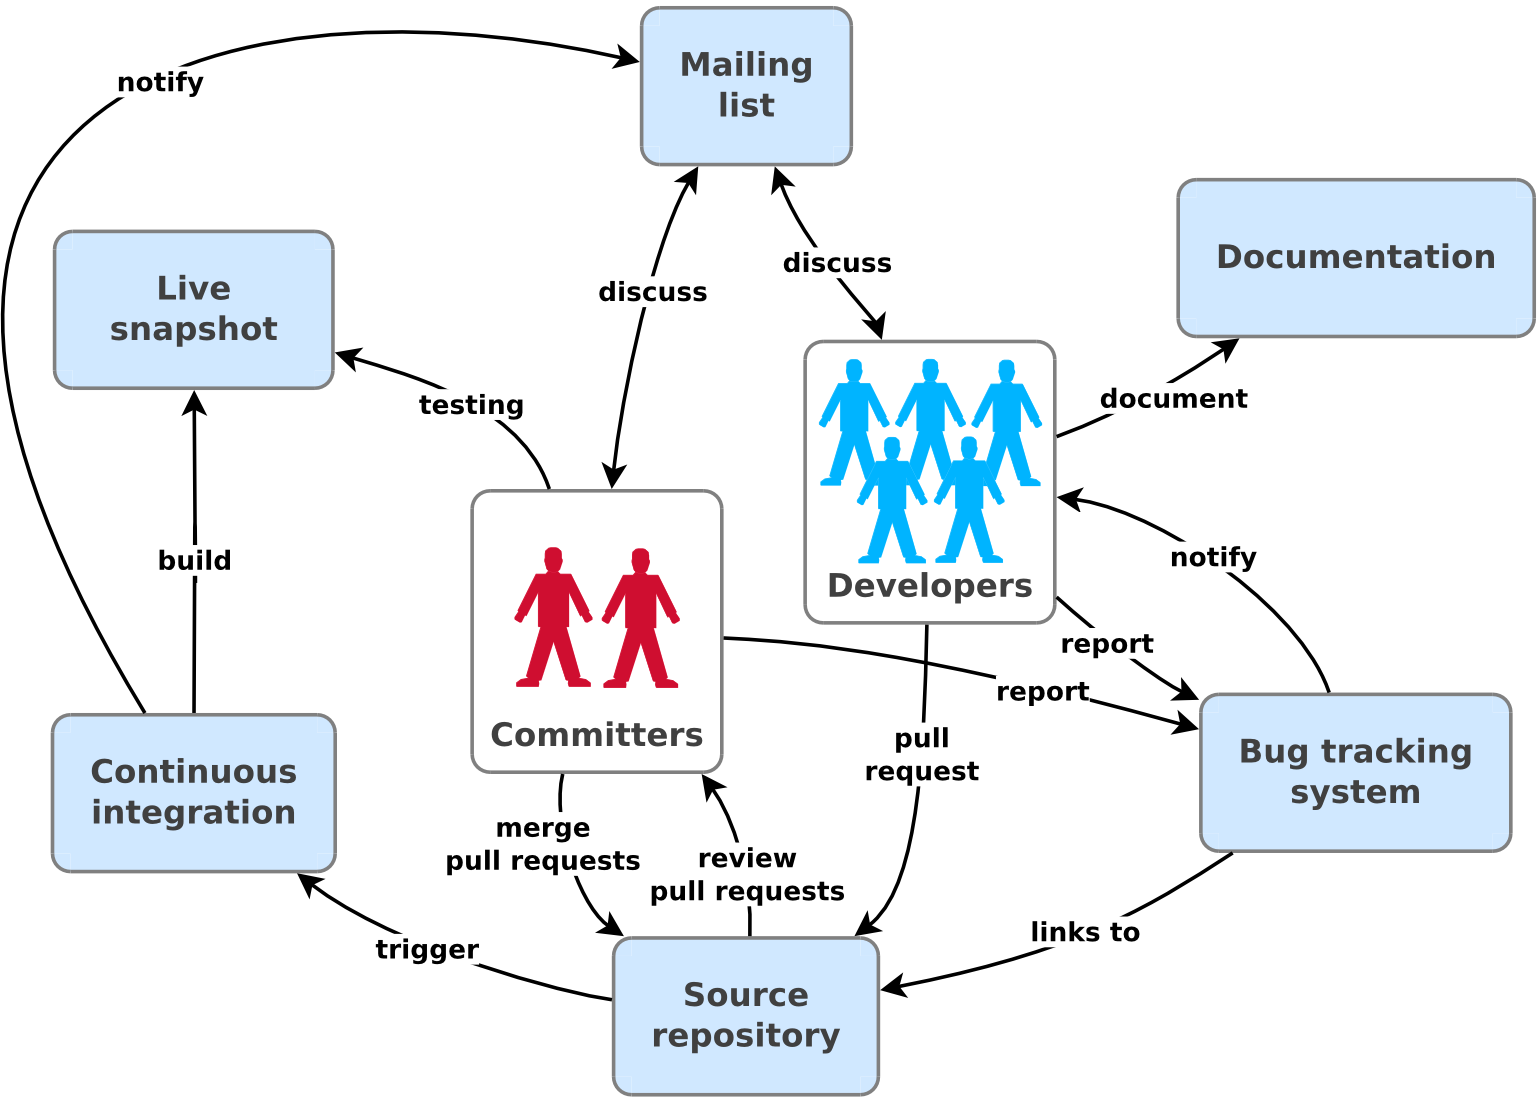
\includegraphics[width=0.67\textwidth]{images/development-workflow.png}
\caption{Development workflow with all tools}
\label{fig:development-workflow}
\end{figure}

\section{Details}
\label{sec:details}

The Figure~\ref{fig:development-workflow} illustrates the global development workflow.
In this workflow, there is two different kind of actors (developers and integrators) which
interact with different kind of tools.
We will now give more details on these tools and how they will be used by the actors.

\subsection{Mailing list}
\label{sec:mailing-list}

An email mailing list will be available for general decision making about the platform,
the goal being to keep records of discussions and choices about developments or architecture design.

\subsection{Source repository}
\label{sec:source-repository}

A distributed source code repository will be provided for storing the source code or binaries
needed for building the \learnpad platform.

Developers will propose new functionality or bug fixing using \emph{pull requests}
\footnote{A pull request is a method of submitting contributions to a software project.
It contains the \emph{patch} representing changes to be made and creates a central place
for those changes to be reviewed and discussed}
which integrators will have the duty to review. An integrator may and accept the
\emph{pull request}, request changes or further information or in an extreme case,
close it pending further discussion.

Despite having direct access to the shared repository, an integrator who is also a developer should
make sure to use \emph{pull requests} for integrating their own functionality so as to allow for
discussion with other integrators and developers and to keep record of the contribution.

All developers should adopt the \emph{check in early and often} development methodology.
Code in development is not expected to be bug-free but great importance is placed on collaboration
and working in the open. In a fast-changing collaborative software development project, frequent
pull requests help everybody. They help the developer making them because he is able to avoid
rewriting code to cope with changes in other elements of the system and they also help other
developers who are able to see and adapt to changes in this developer's component.

\subsection{Documentation}
\label{sec:documentation}

Documentation will be able to be written accompanying the source code in the repository or it
may be places on a provided wiki as long as relevant documents are referenced from the source
repository.

\subsection{Bug tracking system}
\label{sec:bug tracking-system}

All participants will be responsible for discovering and diagnosing of bugs. Bugs, feature
requests and other to-do items shall be reported to a provided bug tracking system where others
will be able to keep track of issues which need to be addressed. Email notifications of new
issues will be sent to integrators and updates of an issue will be sent to those who participate in
(EG: comment on) the issue.

\subsection{Continuous integration}
\label{sec:continuous-integration}

Continuous integration is an automated process by which the current state of the source code is
built into a final product, any automated tests are run and the final product is made available
to developers so that they can test the interaction of their commits in near-real-time. The platform
will be built and deployed on the \emph{target system}, a computer running an installation of
Ubuntu 12.04 LTS \footnote{The stable version of a widely used Linux distribution.}.
Automated builds may also be used as an aid for integrators to do "smoke test" validation on pull
requests before accepting them. In order to protect the working environment of all developers,
it is critical that integrators reject or revert any pull request which causes an incorrect build
of the platform.

\subsection{Live snapshot}
\label{sec:live-snapshot}

Periodically, the most recent build of the \learnpad platform will be automatically published
on a live server running the \emph{target system} so that it can be accessible to all of the
collaborators. This will aid in bug detection and provide a base for discussion of additional
features and the direction of the project.

\chapter{Development process}
\label{ch:development-process}

\section{Documentation}
\label{sec:documentation}

There is a few occasions where documentation is needed: architecture design, deployment process, produced source code, complex algorithms...

\subsection{Architecture design}
\label{sec:architecture-design}

Architectural design needs a lot of discussion before converging.
So the first documentation on that will be contained in the mailing list.
However, this is not a resumed and structured information.
Partners will use at least 2 other medias to improve documentation.

First of all, architecture design imply graphics (for example, UML component diagrams or UML package diagrams).
NME partner is already providing a server where we can collaboratively work on graphics using DrawMagic, a diagram software solution.
It allows us to use a lot of different standardized diagram notations and annotate them; it works as a versionning source repository: everybody can push modifications on it and modifications are merged.

On the other hand, structured and textual documentation about architecture is written on a wiki.
CNR partner already deployed an XWiki instance partly for this goal (and for documenting everything about the \learnpad project in general).

\subsection{Deployment process}
\label{sec:deployment-process}

The deployment of the developed services must be documented on the wiki (already deployed, see Section~\ref{sec:architecture-design}).
However, the deployment will be automatized (as far as possible) for the continuous integration, see Section~\ref{sec:continuous-integration} for more informations.

\subsection{Source code}
\label{sec:source-code}

It exists a lot of supporting tools to document code (Doxygen, JavaDoc, PythonDoc, etc.).
No matter what tool is used, each code should be documented at least at the file level: what the script is for? what the class is for? etc.

\subsection{Complex algorithms}
\label{sec:complex-algorithms}

Some specific parts of source code needs a specific documentation.
Complex algorithms for example, needs a detailed and structured documentation.
Basic source code documentation can be done (see Section~\ref{sec:source-code}) but in these cases, documentation on the wiki or publication of a paper may happen.

\section{Source management}
\label{sec:source-management}

As already said, all source code will be store in a single repository, using a distributed version control system like git, mercurial, Subversion, etc.
To ease the collaboration, each service will takes place in one subdirectory of this main repository.
The source will be published on a public server, and also accessible with an web front-end to ease some of the manipulations (like GitHub, BitBucket, etc.).

\section{Building}
\label{sec:building}

As seen in the Figure~\ref{fig:development-workflow}, a continuous integration will support the development of the platform.
That means that every service should be buildable automatically.
As seen in Source Management (see Section~\ref{sec:source-management}), each service will be a folder in the source repository.
This should allow more freedom in the management of development activities (tools used, subdirectories, etc.).
To ease the global build, each service must provide a file to automatically build it (for example, each folder will contain a \texttt{build.sh} file).
At the root of the repository, a global builder will parse all of the services to build them.
If specific deployment procedures must be done, they should also appear in this build process.

\section{Testing}
\label{sec:testing}

Testing is an important part for the continuous integration.
Unit tests should be developed as the service level; they will help to check the builds and avoid regressions as much as possible.
Integration tests should allow the continuous integration that everything is right during a standard deployment with the last versions of all the services.

For unit tests, each service must provide a way to run the tests (for example, by giving a \texttt{test.sh} file or by allowing a \texttt{test} functionality to the \texttt{build.sh}).
Integration and functional tests are higher levels and should be defined in collaboration.

\section{Bug tracking}
\label{sec:bug-tracking}

Each bug will be tracked with a centralized tool like JIRA, Mantis, GitHub, etc.
The procedure is to report bug each time you encounter problem using services of other partners.
Each partner can also use the tool for reporting its own bugs.
The bug tracking system must be able to notify users by email.

\chapter{Integration plan}
\label{ch:integration-plan}

\section{Releasing process}
\label{sec:releasing-process}

Each month, a version of the platform will be released.
These short releasing deadlines don't expect stable version each time (see Roadmaps in Section~\ref{sec:roadmap}) but at least version without major bugs.
The goal of these short releasing deadlines are:
* make the platform improve step by step
* giving clear and small objectives
* track easily the work
* detect problems early

\section{Roadmap}
\label{sec:roadmap}

There is 2 different kind roadmaps.
\subsection{Global roadmap}
\label{sec:global-roadmap}

A global roadmap of the platform must be provided.
It will be mainly based on the deliverable deadlines with a cycle of multiple unstable release to finally reach a final stable release each 3 months.
This means that each version of the \learnpad platform will go through at the end of the first month milestone; then a release candidate, one month later; and finally, a stable version after 3 months.
This process will cycle during the whole project.

Roadmaps may be rediscussed during the development, considering problems, locks or important changes in architecture for example.
This means that a roadmap must contains a clear view of the next releasing cycle and only guidelines that may be adapted for the releases after.

\subsection{Services roadmaps}
\label{sec:services-roadmaps}

Each service will also have his own roadmap.
These roadmaps will decribes when each functionality must be included in the main \learnpad platform.
Of course, these roadmap will be mapped onto the main roadmap in order to introduce new functionalities during the cycle of the milestone and possibly for the release candidate.
The last month should be reserved for stabilization of the platform.

As for the global roadmap, services roadmaps may be adapted during the process of development.


% ---------------------------------- Bibliography starts here
% ----------------------------------

\bibliographystyle{plain} 
\bibliography{biblio}

\end{document}
